\documentclass [12pt]{article}
\usepackage{graphicx}
\usepackage{amstext,verbatim,alltt}
\usepackage{moreverb}
\setlength{\textwidth}{6.5in}
\setlength{\oddsidemargin}{0in}
\setlength{\evensidemargin}{0in}
\begin{document}

\title{The CacheBench Report}
\author {Philip J. Mucci \\
	Kevin London \\
	John Thurman \\
        {\tt mucci@cs.utk.edu} \\
	{\tt london@cs.utk.edu} \\
	{\tt thurman@cs.utk.edu}}
\date{November 1998}

\maketitle

\section{Introduction}

CacheBench is a benchmark designed to evaluate the performance of the
memory hierarchy of computer systems. Its specific focus is to
parameterize the performance of possibly multiple levels of cache
present on and off the processor. By performance, we mean raw bandwidth
in megabytes per second. Of interest to us is the ability of the cache to 
sustain large, unit-stride, floating point workloads.

\subsection{Cache Architecture}

Caches are essentially very small, high speed memories designed to
speed computation among repeatedly accessed data. They are found on
virtually all commercially available processors from small sixteen bit
embedded microprocessors to the large, multi-million transistor RISC
chips found in today's workstations and supercomputers. Caches exploit
both {\em spatial} and {\em temporal} locality. Spatial locality is 
the concept that
data items that are physically located near each other in main memory
will likely be accessed together. Temporal locality is the concept
that a data item that is frequently accessed will likely be accessed
again in the near future. \\

 When the processor wishes to operate on an item from main memory, it
 issues a load to the cache. If the item is resident in the cache,
 this is called a cache hit. If not, it is called a cache miss, and
 the load request is forwarded to main memory, which moves the data
 from main memory into a cache line. A detailed discussion of cache and processor
 architecture is well beyond the scope of this paper, but interested
 readers are referred to Hennessey and Patterson's, {\em Computer
 Architecture, A Quantitative Approach}. An example in this textbook 
 serves as the basis for this benchmark.

\subsection{Goals of CacheBench}

The goal of this benchmark is to establish peak computation rate given
optimal cache reuse and to verify the effectiveness of high levels of
compiler optimization on tuned and untuned codes.  Many scientific
applications in use have significant resource requirements in terms of
memory footprint. High speedups of these applications are often
achieved through exploiting the cache. This is especially true given
the widening gap between processor speed and main memory. Thus, this
benchmark will provide us with a good basis for application
performance modeling and prediction for those applications that have
already been substantially tuned for cache reuse.

\section{How it works}

CacheBench currently incorporates eight different benchmarks. Each one
 performs repeated access to data items on varying vector
lengths. Timings are taken for each vector length over a number of
iterations. Computing the product of iterations and vector length
gives us the total amount of data accessed in bytes. This total is
then divided by the total time to compute a bandwidth figure. This
figure is in megabytes per second. Here we define a Megabyte as being
$1024^{2}$ or $1048576$ bytes. In addition to this figure, the average
access time in nanoseconds per each data item is computed and reported. 
The tests are as follows.

\begin{itemize}
\item Cache Read
\item Cache Write
\item Cache Read/Modify/Write
\item Hand tuned Cache Read
\item Hand tuned Cache Write
\item Hand tuned Cache Read/Modify/Write
\item memset() from the C library
\item memcpy() from the C library
\end{itemize}

The first six of these tests access their data through arrays of a
predefined base type. This type is set at compile time and defaults to
{\tt double}. The rationale for this is that some systems perform memory
access differently depending on the functional unit that generated the
miss. The default data-type can be altered by setting the {\tt USE\_<type>}
compiler definition in the {\tt Makefile}. Currently {\tt USE\_CHAR}, 
{\tt USE\_INT}, {\tt USE\_FLOAT} and {\tt USE\_DOUBLE} are supported.

The first three of the tests are intended to provide us with
information about how good the compiler is. They are very
straightforward consisting of only a few lines of code.  

The second
three are intended to reflect portable, tuned code as found in
production applications. Here, the optimizer has little opportunity to
enhance the code, and in fact, the numbers from these three tests
often do not change very much given different levels of optimization.

The last two tests are included as points of comparison. These
routines are often heavily used in C applications, but vary greatly in
efficiency. One would expect high performance out of these benchmarks
in terms of memory bandwidth, but more often than not, the results
have been disappointing.

All of these benchmarks runs for a fixed amount of time, which is
tunable at run-time. The rationale for this is the widely varying
performance of processors these days. BLASbench intends to
provide the user with relatively quick feedback about the memory performance
of the machine in use. However, this timing restriction limits the accuracy with which
we can report the results. A faster machine that runs the test for a higher
number of iterations has less relative error. This makes accurate, statistical
analysis difficult but it will be fixed in the next release.

\subsection{Cache Read}

This benchmark is designed to provide us with read bandwidth for
varying vector lengths in a compiler optimized loop. For the cases
where the vector length is less than the cache size, the data will 
come completely from cache and the resulting bandwidth will be much higher.
\\ \ \\
The pseudo code for this test is as follows:

\begin{verbatim}
for all vector length
  timer start
  for iteration count
    for I = 0 to vector length
      register += memory[I] 
  timer stop
\end{verbatim}

\subsection{Cache Write}

This benchmark is designed to provide us with write bandwidth for
varying vector lengths in a compiler optimized loop. This benchmark
is greatly affected by architectural peculiarities in the memory subsystem.
Replacement policy, associativity, blocking and write buffering all play important
factors in the performance of this benchmark. For example, a {\em write-back} cache 
will show a much higher bandwidth because it frequently avoids unnecessary 
references to main memory. In addition, many systems coalesce
and buffer multiple writes to cache/memory. This can hides much of the latency
of the underlying hardware.\\

\begin{verbatim}
for all vector length
  timer start
  for iteration count
    for I = 0 to vector length
      memory[I] = register++
  timer stop
\end{verbatim}

\subsection{Cache Read/Modify/Write}

This benchmark is designed to provide us with read/modify/write bandwidth for
varying vector lengths in a compiler optimized loop. This benchmark generates
twice as much memory traffic, as each data item must be first read from 
memory/cache to register and then back to cache. Each direction of transfer is
counted in the computation of bandwidth. Bandwidth for this test is often a 
bit higher than the sum of the previous two tests. The benefit comes from 
compilers' ability to better schedule operations and group memory accesses
to amortize the cost of the store.

\begin{verbatim}
for all vector length
  timer start
  for iteration count
    for I = 0 to vector length
      memory[I]++ 
  timer stop
\end{verbatim}

\subsection{Hand Tuned Versions}

A full description of the hand tuned versions of these codes is beyond the 
needs of this paper. However,
to provide some background, the following optimizations were applied:

\begin{itemize}
\item Degree eight unrolling. Each loop now references eight memory elements instead of one.
\item Dependency analysis. Each operation is independent of the previous seven.
\item Register re-use. Registers are allocated to memory locations and reused whenever possible.
\end{itemize}

The optimizations reflect what a {\em minimally good} compiler should be doing
on these simple loops. In CacheBench, if we see our compiler loops not
reaching the performance of our tuned loops, we can conclude that our
compiler is poor. The complexity of these loops is minimal and any 
compiler should be able to optimize them. It is possible, that our
compiler optimized loops will outperform our hand-tuned loops, if the
compiler inserts prefetching and coalesces memory operations into
block transfers.

\subsection{Memory Set}

The C library provides us with the function {\tt memset()} to
initialize regions of memory. This function is often highly optimized
as it is widely used both in and outside of the operating
system. Often, this function is either assembly code placed {\em
inline} in the executable from a header file, or it is an {\em
intrinsic} function that the compiler recognizes and replaces
automatically. Some systems have additional hardware on chip to
perform this operation, specifically when the value to be set to is
zero. This benchmark allows us to compare the numbers from our two
formulations of memory write with this version. More often than not, we
find that {\em both versions outperform a call to this routine.}

\begin{verbatim}
for all vector length
  timer start
  for iteration count
    for I = 0 to vector length
      memset(vector1,0xf0,length)
  timer stop
\end{verbatim}

\subsection{Memory Copy}

The C library also provides us with the function {\tt memcpy()} to
copy regions of memory. It is also usually an intrinsic or inline 
assembler function. This benchmark allows us to compare the numbers
from our two versions of memory read/modify/write with this version.
Frequently we find that {\tt memcpy()} is not as fast as it should be.
While this function may not appear explicitly in Fortran application
codes, it is used by many of the supporting libraries, like MPI.

\begin{verbatim}
for all vector lengths
  timer start
  for iteration count
    for I = 0 to vector length
      memcpy(dest,src,vector length)
  timer stop
\end{verbatim}

\section{Using CacheBench}

\subsection{Obtain the Distribution}

BLASBench is now found in the LLCbench distribution.
The latest release of LLCbench can always be found through the original author's homepage at \\
{\tt http://www.cs.utk.edu/$\sim$mucci} \\ at its home page at \\ 
{\tt http://www.cs.utk.edu/$\sim$thurman/llcbench} \\
or via FTP at \\ {\tt ftp://cs.utk.edu/~thurman/pub/llcbench.tar.gz}.\\

Now unpack the installation using {\tt gzip} and {\tt tar}.

\begin{verbatim}
kiwi> gzip -dc llcbench.tar.gz | tar xvf -
kiwi> cd llcbench
kiwi>  ls
Makefile     cachebench/  index.html   mpbench/     sys.def@
blasbench/   conf/        make.def     pix/

\end{verbatim}

\subsection{Build the Distribution}

First we must configure the build for our machine, OS and BLAS libraries. All
configurations support the reference BLAS if available. Before configuration 
{\tt make} with no arguments lists the possible targets.

\begin{verbatim}
kiwi> make
Please use one of the following targets:

        solaris sunos5
        sun sunos4
        sgi-o2k o2k
        linux-mpich
        linux-lam
        alpha
        t3e
        ppc ibm-ppc
        pow2 ibm-pow2
        reconfig (to bring this menu up again)

After configuration, please check the VBLASLIB variable in 
sys.def and make sure that it is pointing to the vendor BLAS
library if one exists.

\end{verbatim}

Configure the build. Here, we are on a Solaris workstation.

\begin{verbatim}
kiwi> make solaris
ln -s conf/sys.solaris sys.def

\end{verbatim}

CacheBench's default runtime variable values are contained in the file {\tt make.def} and may
be modified there.

\subsection{Building CacheBench}

\begin{verbatim}

kiwi> make cache-build
cd cachebench; make cachebench
cc -fast -dalign -DREGISTER -DUSE_DOUBLE -c cachebench.c 
cc  -DUSE_DOUBLE -o cachebench cachebench.o 

\end{verbatim}

\subsection{Running CacheBench}

While CacheBench can be run from the command line, it is designed executed
through use of the {\tt Makefile}. The resulting datafiles for each of the runs 
will be left in the file: \\
{\tt results/<test>-<HOSTNAME>-<DATATYPE>.dat}. \\

\begin{verbatim}
kiwi> make cache-run
Measuring Read...
Measuring Write...
Measuring RMW...
Measuring Tuned Read...
Measuring Tuned Write...
Measuring Tuned RMW...
Measuring memcpy()...
Measuring memset()...
.
[commands deleted for brevity].
.
\end{verbatim}

\subsection{CacheBench results}

{\tt make cache-graphs} will attempt to graph
the results. The datafiles willl be tarred into a file called {\tt cacheperf-<HOSTNAME>-<DATATYPE>.tar}.
The {\tt Makefile} will then attempt to graph the results.
If {\tt GNUPlot} is not available on this system, simply copy
{\tt cacheperf-<HOSTNAME>-<DATATYPE>.tar} to another machine that has
{\tt GNUPlot}, extract the tar file and process each {\tt GNUPlot} script file
with {\tt gnuplot < <HOSTNAME>.gp > <file>.ps}.

\begin{verbatim}
kiwi> make cache-graphs
cd cachebench; make graphs
.
.
.
X=`uname -n`; cd results; gnuplot < $X.gp > cacheperf-$X-DOUBLE.ps

If you don't have GNUplot, you can make the graphs on another machine
using the cachebench/results/cacheperf-cetus3b-DOUBLE.tar file.
\end{verbatim}

\subsection{Arguments to CacheBench}

This is the CacheBench arguement list from the command line help.  The defaults listed are
for direct execution of the benchmark (not the defaults for execution through the makefile).

\begin{verbatim}
Usage: cachebench -rwbtsp [-x #] [-m #] [-d #] [-e #]
         -r Read benchmark
         -w Write benchmark
         -b Read/Modify/Write benchmark
         -t Use hand tuned versions of the above
         -s memset() benchmark
         -p memcpy() benchmark
         -x Number of measurements to take between powers of 2
         -m Specify the log base 2 of the available physical memory
         -d Number of seconds per iteration
         -e Number of times to repeat test for each vector size

Datatype used is double, 8 bytes
Defaults if  tty: -rwbsp -x1 -m24 -d5 -e2
Defaults if file: -b   -x1 -m24 -d5 -e1
\end{verbatim}

Note the fact that the defaults are different depending on whether or not the
output is directed to a TTY or a file. Again, the best way to run cachebench
is with the {\tt Makefile}.

\clearpage
\newpage

\section{Results on the CEWES MSRC Machines}

The following graphs are taken from our runs on each of the CEWES
MSRC machines during dedicated time. Those machines are the SGI Origin
2000, the IBM SP and the Cray T3E. The cache size and theoretical 
peak MFLOPS for each machine are listed as follows. The peak MFLOPS
is as reported by the vendor and is simply computed as a product of 
the clock speed times the number of independent FMA's that can be
computed per cycle.

\begin{center}
\begin{tabular}{|l|l|r|} \hline
{\em Machine} & {\em Cache } & {\em Peak}\\ \hline
SGI Origin 2000 & 32K,4MB & 390 \\ \hline
IBM SP & 128K & 240 \\ \hline
Cray T3E & 8K,96K & 900 \\ \hline
\end{tabular}
\end{center}

\clearpage
\newpage

\subsection{Cache Reads}
\begin{figure}[Hht]
\centerline{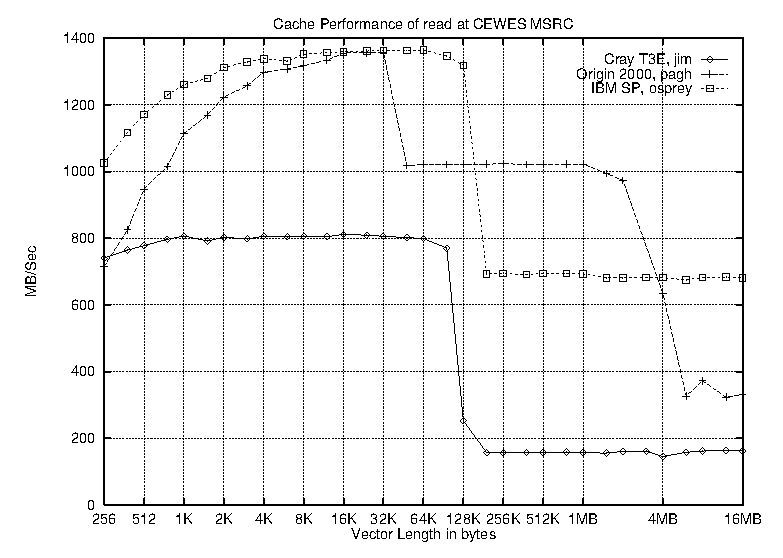
\includegraphics{pics/cache_cewes_read.ps}}
\caption{Performance of Compiler Optimized Memory Read}\label{read}
\end{figure}

\begin{figure}[Hht]
\centerline{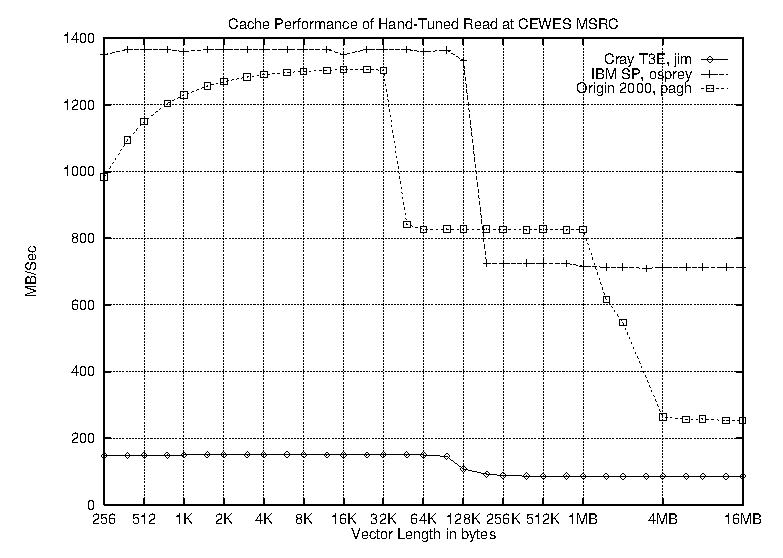
\includegraphics{pics/cache_cewes_handread.ps}}
\caption{Performance of Hand-tuned Memory Read}\label{handread}
\end{figure}

In figures \ref{read} and \ref{handread}, we notice that the read
performance of the Cray T3E is much lower for the hand-tuned
version. For the compiler optimized version, we find a two to 
threefold improvement for vector sizes that lie in cache. The Cray compiler
seems to have a very difficult time recognizing what optimized code is doing.
This means that tuned applications ported to the Cray {\em might not perform
very well}. For the SP2 and the Origin 2000,
the only difference we find is the steepness of the portion of the
curve lying substantially below the cache size.  Here, we are seeing
the overhead of the compiler's code that handles the special cases
where the vector length is not a multiple of the degree of
unrolling. In the tuned version, this {\em residual} code does not
exist and thus there are no branches in the underlying assembly
language. The SP has a hardware loop capability allowing zero cycle
branches. For the hand-tuned version, there is no residual code, so the
compiler simply sets up the hardware loop and lets it run with no overhead.
Thus, we see no performance falloff at smaller vector lengths. 

\clearpage
\newpage

\subsection{Cache Writes}
\begin{figure}[Hht]
\centerline{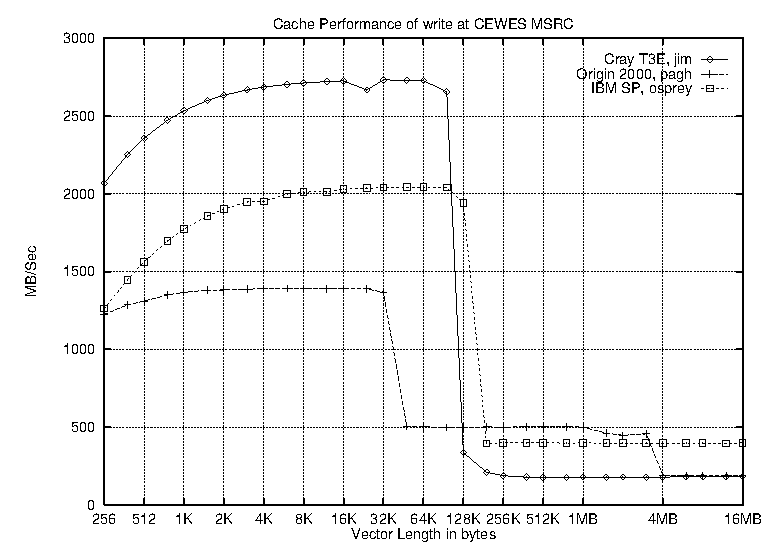
\includegraphics{pics/cache_cewes_write.ps}}
\caption{Performance of Compiler Optimized Memory Write}\label{write}
\end{figure}

\begin{figure}[Hht]
\centerline{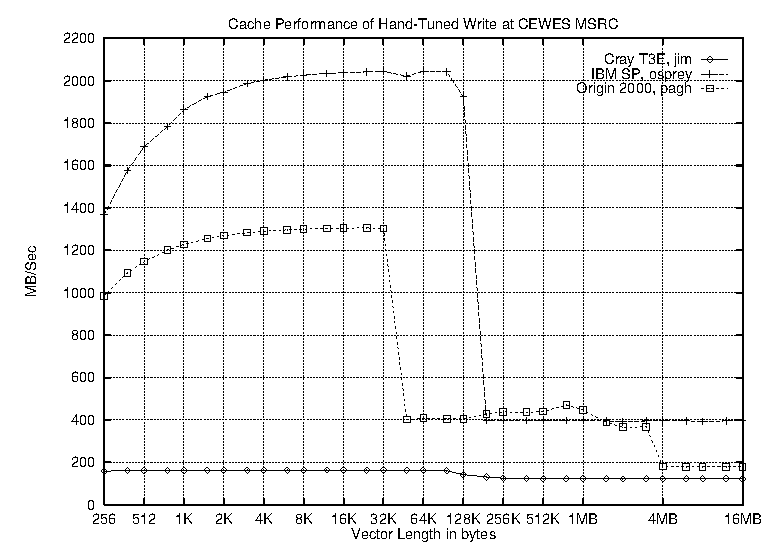
\includegraphics{pics/cache_cewes_handwrite.ps}}
\caption{Performance of Hand-tuned Memory Write}\label{handwrite}
\end{figure}

In figures \ref{write} and \ref{handwrite}, we can see that the performance of
the compiler optimized loop is equal to or greater than that of the hand 
tuned loop as is the case for reads.
The reader will notice that for vectors residing completely in L1 cache,
the write bandwidth is equal to or greater than the read bandwidth. On the
Origin, the L2 cache is significantly slower to write to than to read from. 
We infer that the compiler is probably prefetching on the read case
and that there is inadequate pipelining between L2 cache and memory. For the
T3E, we again notice how poorly the compiler does on the optimized code.

\clearpage
\newpage

\subsection{Cache Read/Modify/Write}
\begin{figure}[Hht]
\centerline{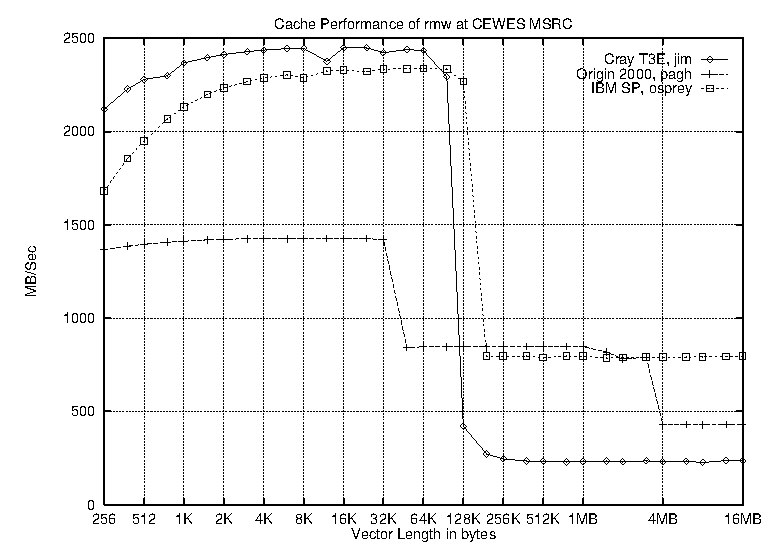
\includegraphics{pics/cache_cewes_rmw.ps}}
\caption{Performance of Compiler Optimized Memory Read/Modify/Write}\label{rmw}
\end{figure}

\begin{figure}[Hht]
\centerline{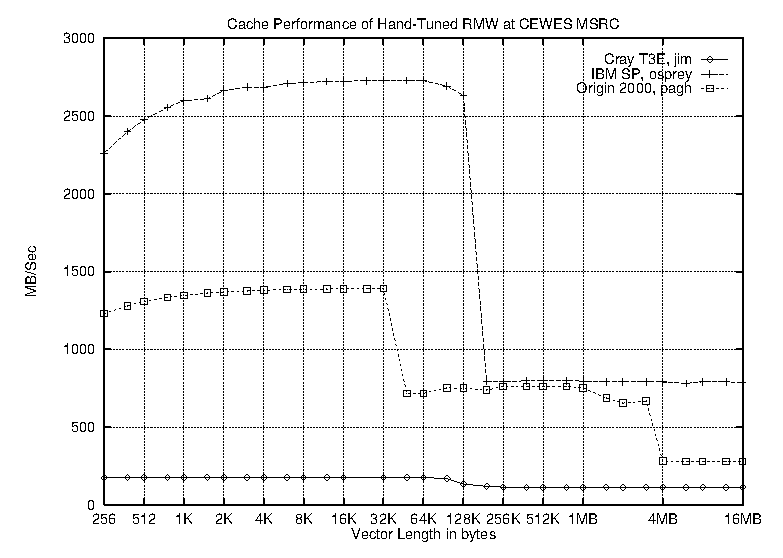
\includegraphics{pics/cache_cewes_handrmw.ps}}
\caption{Performance of Hand-tuned Memory Read/Modify/Write}\label{handrmw}
\end{figure}

Of interest in figure\ref{rmw} and \ref{handrmw} is the difference 
in performance of the IBM
SP. Note that in the hand-tuned version, performance averages about six 
hundred megabytes per second better than that of the compiler optimized
version. In the tuned version, the compiler is probably scheduling/aggregating
memory access
into double-word loads and stores, a unique feature of this architecture. This probably happens in the compiler
optimized version, but the fact that the compiler must also unroll the loop 
and optimize register usage seems to complicate its analysis. Also of interest is the better
performance on the T3E in level two cache for the untuned version. {\em Software
pipelining}, the mixing instructions from one iteration to another may
be aiding this code to hide the latency of the level two cache misses. We
are seeing this behavior in the case for reads and writes as well.

\clearpage
\newpage

\subsection{{\tt memset()}}
\begin{figure}[Hht]
\centerline{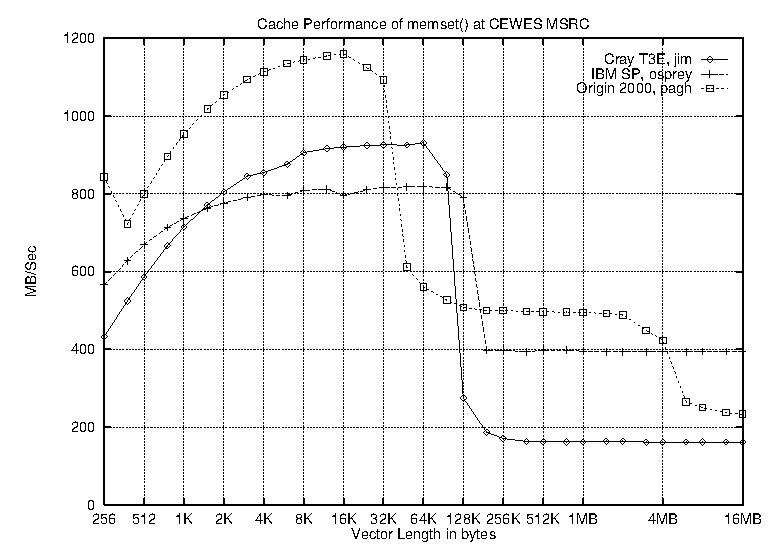
\includegraphics{pics/cache_cewes_memset.ps}}
\caption{Performance of {\tt memset()}}\label{memset}
\end{figure}

\subsection{{\tt memcpy()}}
\begin{figure}[Hht]
\centerline{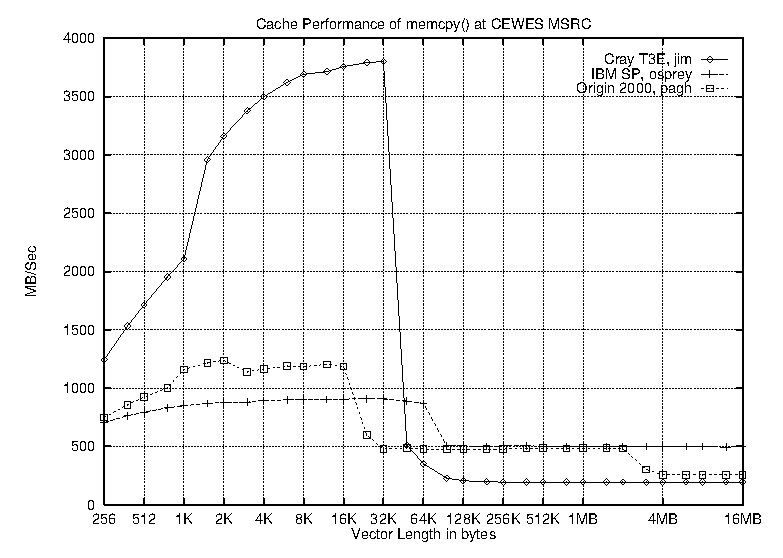
\includegraphics{pics/cache_cewes_memcpy.ps}}
\caption{Performance of {\tt memcpy()}}\label{memcpy}
\end{figure}

Figures \ref{memset} and \ref{memcpy} are provided as reference. The
performance of these two routines, when compared with the write and read-modify-write benchmark, clearly indicates that the user
would be better off using a {\em typed} version coded in C or Fortran
rather than these library calls. The reason for this is that they are
often coded at the byte level for maximum flexibility, not
performance. By knowing the type and the alignment of the data ahead of
time, the user could easily write a simple loop, let the compiler
optimize it and still see much better performance. The only exception
is the case where the vector is smaller than L2 cache on the T3E.

\clearpage
\newpage

\section{Future work}

\begin{itemize}
\item Provide option for measuring specific vector lengths.
\item Use specialized, high-resolution timers where available.
\item Add benchmark for pointer traversal to measure latency of cache hit 
and miss.
\item Add parameters to tune the placement and padding of the vectors.
\item Change from constant run-time to constant iterations.
\item Add unoptimized, untuned case for a baseline.
\item Standardize configuration with GNU {\em autoconf}.
\item Grab machine configuration and store it with each run.
\item Standardize data/graph naming scheme with timestamp.
\end{itemize}

\section{References}

{\em Computer Architecture, A Quantitative Approach} by David A. Patterson, John L. Hennessy, David Goldberg,
Softcover, 1050 Pages, Published by Morgan Kaufmann Publishing, 01/1996, ISBN: 1558603298 \\ \ \\
{\em The Science of Computer Benchmarking (Software, Environments, Tools)} by Roger W. Hockney,
Softcover, 600 Pages, Published by Society for Industrial and Applied, 6/1996, ISBN: 0898713633

\end{document}
